\documentclass[aspectratio=169]{beamer}

% ---------- THEME & LOOK ----------
\usetheme{Madrid}
\usecolortheme{seahorse}
\usefonttheme{professionalfonts}
\setbeamertemplate{navigation symbols}{}
\setbeamercovered{transparent}
\setbeamertemplate{itemize items}[circle]
\setbeamertemplate{enumerate items}[default]
\setlength{\parskip}{0.25em}

% ---------- COLORS ----------
\usepackage{xcolor}
\definecolor{accent}{RGB}{0,92,184}
\definecolor{soft}{RGB}{233,244,255}
\setbeamercolor{structure}{fg=accent}
\setbeamercolor{title}{fg=white,bg=accent}
\setbeamercolor{frametitle}{fg=accent}
\setbeamercolor{block title}{bg=accent!10,fg=accent}
\setbeamercolor{block body}{bg=soft}

% ---------- PACKAGES ----------
\usepackage{booktabs}
\usepackage{amsmath, amssymb}
\usepackage{array}
\usepackage{graphicx}
\usepackage{hyperref}
\hypersetup{colorlinks=true,linkcolor=accent,urlcolor=accent}

% ---------- PLACEHOLDER BOX ----------
\newcommand{\placeholderbox}[2][0.82\linewidth]{%
  \begin{center}
    \fbox{\begin{minipage}[c][0.46\textheight][c]{#1}
      \centering \vspace{0.25em}
      \textbf{#2}\\[0.6em]
      \emph{Insert figure/table here later.}
    \end{minipage}}
  \end{center}
}

% ---------- TITLE ----------
\title{\textbf{Discrimination and Male--Female Earnings Differentials}}
\subtitle{{\large ECON 300 - Labour Economics}}
\author{Muhebullah Karimzada}
\date{Winter 2026}

\begin{document}

% ============================================================
% TITLE
% ============================================================
\begin{frame}[plain]
  \titlepage
\end{frame}

% ============================================================
\section{Orientation}
% ============================================================

\begin{frame}{Learning Objectives}
\transfade
\begin{itemize}[<+->]
  \item Describe the factors giving rise to male--female pay gaps and the role of discrimination.
  \item Outline methodologies used to estimate discriminatory pay gaps and their challenges.
  \item Explain how discriminatory gaps can persist even with competitive pressures.
  \item Discuss pros and cons of policy initiatives to combat discrimination.
  \item Explain the evolution of the gender pay gap and the mechanics of pay equity.
\end{itemize}

\begin{block}{Interpretation}
This chapter separates \textbf{observed wage differences} from \textbf{true discrimination}. Not every pay gap is discriminatory; some may reflect differences in experience, occupation, hours, or job interruptions.
\end{block}
\end{frame}

\begin{frame}{Main Questions}
\transfade
\begin{itemize}[<+->]
  \item How can equally productive men and women be paid different wages in competitive markets?
  \item Will competitive forces dissipate discrimination?
  \item How do we measure discrimination credibly in the data?
  \item How much discrimination exists in Canada? What about other groups?
  \item Which policies have been adopted, and which are effective?
\end{itemize}

\begin{exampleblock}{Example}
If a man and a woman with the same schooling, experience, and job duties are paid differently, economists ask whether the difference comes from unmeasured productivity, job choice, or discrimination.
\end{exampleblock}
\end{frame}

% ============================================================
\section{Definition and Theory Map}
% ============================================================

\begin{frame}{What is Labour-Market Discrimination?}
\transfade
\begin{block}{Definition}
\textbf{Labour-market discrimination} is unequal treatment of groups with the same productivity, or the same productivity-related traits.
\end{block}

\begin{itemize}[<+->]
  \item \textbf{Employers} may discriminate through wages, hiring, assignments, or promotions.
  \item \textbf{Co-workers} may discriminate because of prejudice, misinformation, or job-security concerns.
  \item \textbf{Customers} may have discriminatory preferences that firms respond to.
\end{itemize}

\begin{block}{Key Distinction}
A \textbf{pay gap} is not automatically discrimination. A gap becomes discrimination when equally productive workers are treated differently because of group identity.
\end{block}
\end{frame}

\begin{frame}{Theory Map}
\transfade
\begin{itemize}[<+->]
  \item \textbf{Demand theories}
  \item \textbf{Supply theories}
  \item \textbf{Noncompetitive theories}
  \item \textbf{Queuing and efficiency-wage considerations}
\end{itemize}

\begin{block}{Interpretation}
These theories explain why wage gaps may arise, why they may persist, and why market competition alone may not fully eliminate them.
\end{block}
\end{frame}

% ============================================================
\section{Demand Theories}
% ============================================================

\begin{frame}{Demand Theories of Discrimination}
\transfade
\begin{itemize}[<+->]
  \item Lower demand for female labour implies lower wages and employment.
  \item Possible channels:
  \begin{itemize}[<+->]
    \item underestimation of female productivity
    \item statistical discrimination
    \item signalling stories
  \end{itemize}
\end{itemize}

\begin{block}{Definition: Statistical Discrimination}
Employers use group averages as a shortcut when they cannot perfectly observe individual productivity.
\end{block}

\begin{exampleblock}{Example}
If employers incorrectly believe women are more likely to leave the labour force, they may offer lower wages even to women who plan to stay continuously employed.
\end{exampleblock}
\end{frame}

\begin{frame}{Interpretation of Demand-Side Discrimination}
\transfade
\begin{itemize}[<+->]
  \item If employers perceive a group as less productive, the labour demand curve for that group shifts left.
  \item This reduces both equilibrium wages and employment.
  \item Even if the beliefs are false, the wage gap can persist if employers act on them.
\end{itemize}

\begin{block}{Economic Intuition}
Demand-side discrimination operates like a reduction in the perceived marginal revenue product of the targeted group.
\end{block}
\end{frame}

% ============================================================
\section{Supply Theories}
% ============================================================

\begin{frame}{Supply Theories of Discrimination}
\transfade
\begin{itemize}[<+->]
  \item Increased supply of female labour can depress wages if productivity or matching suffers.
  \item \textbf{Crowding hypothesis:} segregation into ``female-type'' jobs creates excess labour supply in those occupations, lowering wages.
  \item \textbf{Dual labour market:} men may be concentrated in core jobs and women in secondary-sector jobs with lower wages.
\end{itemize}

\begin{block}{Definition: Crowding}
\textbf{Crowding} occurs when barriers restrict one group to a narrow set of jobs, increasing labour supply there and pushing wages down.
\end{block}
\end{frame}

\begin{frame}{Examples of Supply-Side Mechanisms}
\transfade
\begin{itemize}[<+->]
  \item If women are discouraged from entering engineering, more women may end up in clerical or care-sector jobs, increasing labour supply there.
  \item This can lower wages in female-dominated occupations even when productivity is not lower.
  \item Occupational segregation may therefore create a wage gap without direct employer prejudice in a single firm.
\end{itemize}

\begin{exampleblock}{Example}
If nursing and elementary teaching become heavily female-dominated while skilled trades remain male-dominated, relative wages may diverge because labour is unevenly distributed across occupations.
\end{exampleblock}
\end{frame}

% ============================================================
\section{Noncompetitive and Queuing Theories}
% ============================================================

\begin{frame}{Noncompetitive \& Queuing Theories}
\transfade
\begin{itemize}[<+->]
  \item \textbf{Noncompetitive theories:} adjustment costs and imperfect information can sustain wage gaps.
  \item \textbf{Queuing / Efficiency-wage theories:} firms may pay above-market wages to reduce turnover, increase morale, or raise effort.
  \item Queues for good jobs can interact with gender differences and reinforce unequal outcomes.
\end{itemize}

\begin{block}{Interpretation}
When wages are not fully flexible or information is imperfect, discrimination can persist longer than simple competitive models suggest.
\end{block}
\end{frame}

\begin{frame}{Why Competition May Not Eliminate Discrimination}
\transfade
\begin{itemize}[<+->]
  \item In a simple Becker-style model, discriminatory firms should lose profits and eventually shrink.
  \item In practice, labour markets are not perfectly competitive.
  \item Search frictions, mobility costs, imperfect information, and institutional barriers slow adjustment.
\end{itemize}

\begin{block}{Key Point}
Competitive pressure may reduce discrimination, but it does not guarantee its disappearance.
\end{block}
\end{frame}

% ============================================================
\section{Productivity Differences}
% ============================================================

\begin{frame}{Productivity Differences: Choice or Discrimination?}
\transfade
\begin{itemize}[<+->]
  \item Differences in acquired human capital may reflect:
  \begin{itemize}[<+->]
    \item shorter expected labour-force attachment
    \item higher turnover or absenteeism
    \item household and caregiving responsibilities
  \end{itemize}
\end{itemize}

\begin{block}{Interpretation}
Observed wage gaps may partly reflect differences in experience or job continuity, but these differences themselves may be shaped by social norms and constraints.
\end{block}
\end{frame}

\begin{frame}{Choice, Constraints, and Discrimination}
\transfade
\begin{itemize}[<+->]
  \item Some differences are often presented as ``choices,'' but choices are made within constraints.
  \item Caregiving responsibilities, lack of childcare, and social expectations can affect experience and occupational choice.
  \item Therefore, the boundary between ``choice'' and discrimination is often blurry.
\end{itemize}

\begin{exampleblock}{Example}
If women take more career interruptions because childcare is costly or unavailable, the resulting wage gap is partly tied to institutions, not just preferences.
\end{exampleblock}
\end{frame}

% ============================================================
\section{Oaxaca-Blinder}
% ============================================================

\begin{frame}{Setup: Oaxaca(-Blinder) Decomposition}
\transfade
Let
\[
\ln W = X\beta + \varepsilon
\]
be estimated separately for men and women.

Then the mean log wage gap can be decomposed as:
\[
\ln W_m - \ln W_f
=
(\bar X_m - \bar X_f)'\hat{\beta}_m
+
\bar X_f'(\hat{\beta}_m - \hat{\beta}_f)
\]

\begin{itemize}[<+->]
  \item First term: part \textbf{explained} by differences in characteristics.
  \item Second term: \textbf{coefficient effect} or unexplained gap, often interpreted as discrimination.
  \item The decomposition depends on the chosen reference wage structure.
\end{itemize}
\end{frame}

\begin{frame}{Definition and Interpretation of Oaxaca Decomposition}
\transfade
\begin{block}{Definition}
The \textbf{Oaxaca-Blinder decomposition} is a method for splitting an average wage gap into:
\begin{itemize}
  \item a part due to differences in measured characteristics, and
  \item a residual part due to differences in returns to those characteristics.
\end{itemize}
\end{block}

\begin{block}{Interpretation}
The unexplained component is not automatically pure discrimination, but it is often used as a benchmark estimate of discriminatory treatment.
\end{block}
\end{frame}

\begin{frame}{Figure 12.1: Graphical Illustration of the Oaxaca Decomposition}
\centering
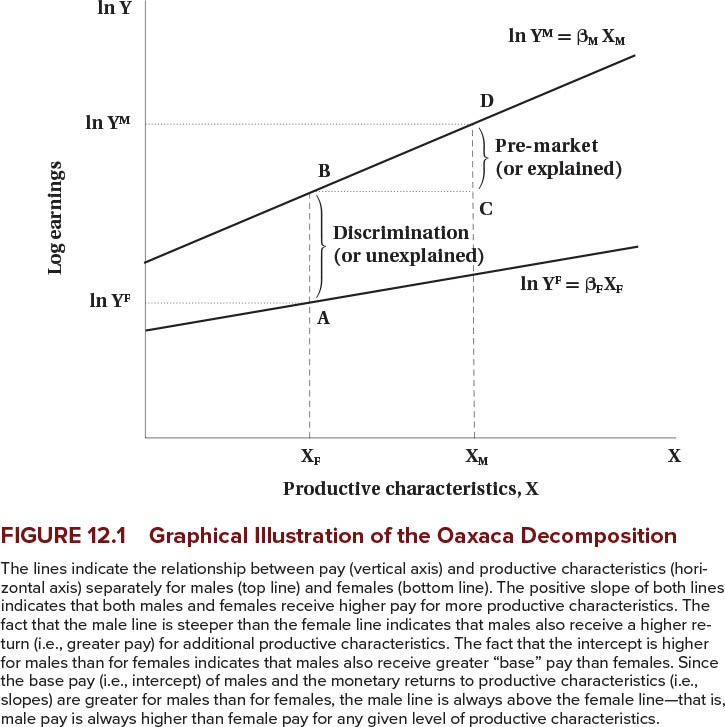
\includegraphics[width=0.72\linewidth]{ben54842_1201}
\end{frame}

\begin{frame}{Reading Figure 12.1}
\transfade
\begin{itemize}[<+->]
  \item The vertical axis is log earnings; the horizontal axis is productive characteristics \(X\).
  \item One wage equation is estimated for men and another for women.
  \item The total wage gap can be split into:
  \begin{itemize}[<+->]
    \item an \textbf{explained} or pre-market part from different characteristics,
    \item an \textbf{unexplained} part from different coefficients.
  \end{itemize}
\end{itemize}

\begin{block}{Key Idea}
If men and women had the same productive characteristics, any remaining gap is interpreted as evidence of unequal returns.
\end{block}
\end{frame}

\begin{frame}{Worked Example: Determinants of Earnings}
\transfade
Estimated earnings equations:

\[
\ln W_m = 0.40 + 0.07S + 0.06EXP + 0.05Married + 0.01Children
\]

\[
\ln W_f = 0.01 + 0.10S + 0.04EXP - 0.02Married - 0.05Children
\]

Group means:
\[
\bar X_m = (S=14, EXP=10, M=0.5, C=0.6), \quad
\bar X_f = (S=15, EXP=7, M=0.5, C=0.6)
\]

\begin{block}{Goal}
Use these equations to compute the raw gap and counterfactual outcomes.
\end{block}
\end{frame}

\begin{frame}{Worked Example: Predicted Values and Raw Gap}
\transfade
Predicted male log wage:
\[
E(\ln W_m)=0.40+0.07(14)+0.06(10)+0.05(0.5)+0.01(0.6)=2.01
\]

Predicted female log wage:
\[
E(\ln W_f)=0.01+0.10(15)+0.04(7)-0.02(0.5)-0.05(0.6)=1.75
\]

Raw female-to-male ratio:
\[
\frac{E(\ln W_f)}{E(\ln W_m)}=\frac{1.75}{2.01}\approx 0.87
\]

\begin{block}{Interpretation}
Women in this example are predicted to earn about 87\% of men's predicted log earnings.
\end{block}
\end{frame}

\begin{frame}{Worked Example: Counterfactual Pay Structures}
\transfade
Female characteristics evaluated at male coefficients:
\[
\ln W_f^* = 0.40 + 0.07(15)+0.06(7)+0.05(0.5)+0.01(0.6)=1.90
\]

Male characteristics evaluated at female coefficients:
\[
\ln W_m^* = 0.01 + 0.10(14)+0.04(10)-0.02(0.5)-0.05(0.6)=1.77
\]

Implications:
\[
\ln W_f^* - E(\ln W_m)=1.90-2.01=-0.11
\]
\[
E(\ln W_f)-\ln W_m^*=1.75-1.77=-0.02
\]

\begin{block}{Interpretation}
Counterfactuals help answer: \emph{What would women earn if they were paid according to the male pay structure?}
\end{block}
\end{frame}

% ============================================================
\section{Evidence}
% ============================================================

\begin{frame}{Additional Evidence on Male--Female Pay Differentials}
\transfade
\begin{itemize}[<+->]
  \item Studies examine wage, sex, institutional, and household discrimination channels.
  \item Average female earnings are often reported below male earnings in some datasets and periods.
  \item Key question: What would women earn if they were treated like men while holding productive traits fixed?
\end{itemize}

\begin{block}{Examples of Channels}
Glass ceilings, interrupted careers, occupational segregation, and differential promotions can all contribute to observed gaps.
\end{block}
\end{frame}

\begin{frame}{Empirical Evidence for Other Groups}
\centering
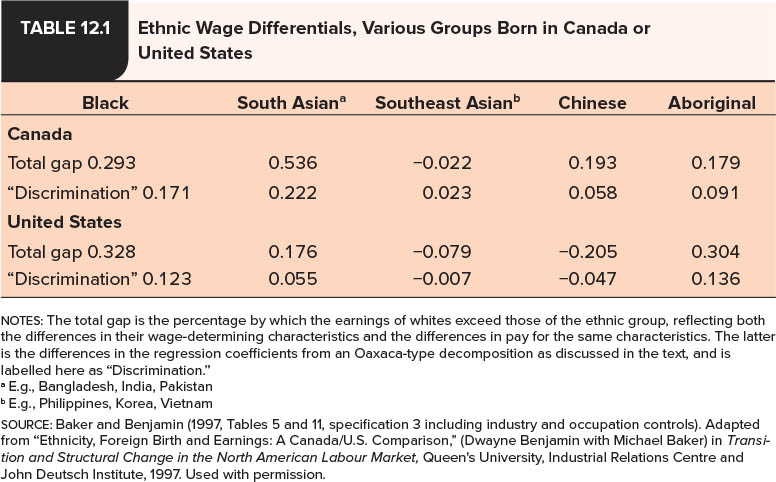
\includegraphics[width=1\linewidth]{ben54842_tb1201}
\end{frame}

\begin{frame}{How to Read Table 12.1}
\transfade
\begin{itemize}[<+->]
  \item The \textbf{total gap} measures the overall difference in wages relative to the reference group.
  \item The \textbf{discrimination} column reports the unexplained component after controlling for measured characteristics.
  \item The gap can differ across countries and groups because institutions, labour markets, and histories differ.
\end{itemize}

\begin{block}{Interpretation}
A positive unexplained gap suggests lower pay than expected given observed characteristics.
\end{block}
\end{frame}

% ============================================================
\section{Policy Toolkit}
% ============================================================

\begin{frame}{Policy Toolkit}
\transfade
\begin{itemize}[<+->]
  \item \textbf{Conventional equal pay:} same job, same establishment.
  \item \textbf{Equal value / Pay equity / Comparable worth:} compare predominantly male and female jobs of equal value.
  \item \textbf{Equal employment opportunity (EEO):} protect against discrimination in recruiting, hiring, and promotion.
  \item \textbf{Affirmative action / Employment equity:} targeted plans for designated groups.
  \item \textbf{Facilitating policies:} childcare and family-friendly practices.
\end{itemize}
\end{frame}

\begin{frame}{Definitions of the Main Policy Tools}
\transfade
\begin{block}{Equal Pay}
Equal pay for the same work in the same establishment.
\end{block}

\begin{block}{Pay Equity / Comparable Worth}
Equal pay for jobs of \textbf{equal value}, even if the jobs are different.
\end{block}

\begin{block}{EEO}
Rules and institutions aimed at preventing discrimination in access to jobs and advancement.
\end{block}
\end{frame}

\begin{frame}{Equal Pay and Pay Equity}
\transfade
\begin{itemize}[<+->]
  \item Equal pay legislation requires equal pay for equal value within the same establishment.
  \item Job evaluation must be free of gender bias.
  \item All Canadian jurisdictions except Alberta have some relevant legislation.
\end{itemize}

\begin{block}{Interpretation}
Equal pay is narrower than pay equity. Equal pay compares similar jobs; pay equity can compare different jobs judged to be of equal value.
\end{block}
\end{frame}

\begin{frame}{Comparable Worth: Design Features}
\transfade
\begin{itemize}[<+->]
  \item Define gender predominance.
  \item Choose a job-evaluation procedure.
  \item Specify adjustment procedures and possible exemptions.
  \item Enforcement and complaint mechanisms matter in practice.
\end{itemize}

\begin{exampleblock}{Example}
A hospital may compare compensation for a male-dominated technical occupation with a female-dominated care occupation and adjust wages if the jobs are evaluated as equal in value.
\end{exampleblock}
\end{frame}

\begin{frame}{EEO and Employment Equity}
\transfade
\begin{itemize}[<+->]
  \item \textbf{EEO} can raise female employment and wages by reducing barriers in recruiting, hiring, and promotion.
  \item \textbf{Employment equity} in federal jurisdiction applies to designated groups including:
  \begin{itemize}[<+->]
    \item women,
    \item visible minorities,
    \item persons with disabilities,
    \item Aboriginal peoples.
  \end{itemize}
\end{itemize}

\begin{block}{Interpretation}
These policies aim not only to equalize wages but also to improve access to better jobs.
\end{block}
\end{frame}

\begin{frame}{Facilitating Policies}
\transfade
\begin{itemize}[<+->]
  \item Childcare support
  \item Parental leave
  \item Flexible scheduling
  \item Family-friendly workplace practices
\end{itemize}

\begin{block}{Interpretation}
These policies do not directly set wages, but they can reduce structural constraints that generate wage gaps.
\end{block}

\begin{exampleblock}{Example}
Affordable childcare may increase continuous labour-force attachment and reduce experience gaps between men and women.
\end{exampleblock}
\end{frame}

% ============================================================
\section{Impact and Summary}
% ============================================================

\begin{frame}{Overall Impact}
\transfade
\begin{itemize}[<+->]
  \item Equal pay and EEO show mixed evidence on broad wage-gap closure.
  \item Comparable worth appears to reduce gaps where implemented.
  \item Policy effects can be limited by scope, design, and enforcement.
\end{itemize}

\begin{block}{Key Point}
Policy matters, but implementation quality matters just as much as legislation itself.
\end{block}
\end{frame}

\begin{frame}{Summary}
\transfade
\begin{itemize}[<+->]
  \item Labour-market discrimination is unequal treatment of equally productive workers.
  \item Demand, supply, noncompetitive, and queuing theories provide different explanations for wage gaps.
  \item Oaxaca-type decompositions separate explained from unexplained wage differences.
  \item Evidence shows persistent gender and group differentials.
  \item Policy tools include equal pay, pay equity, EEO, employment equity, and facilitating policies.
\end{itemize}


\end{frame}

\begin{frame}
\centering
\Huge{\textbf{Thank You!}}
\end{frame}

\end{document}